\documentclass{article}[18pt]
\usepackage{../../../../../format}
\lhead{CT - Graphs}


\begin{document}
\begin{center}
\underline{\huge Randomised Algorithms II}
\end{center}
\section{Randomised algorithms}
\begin{itemize}
	\item The behaviour of a randomised algorithm is influenced by random decisions
	\item If it runs many times with the same input it has different outputs/running times
	\item Why randomised algorithms?
	\begin{itemize}
		\item they are usually simpler to devise
		\item and run faster than deterministic ones
	\end{itemize}
	\item Las Vegas algorithms:
	\begin{itemize}
		\item Always find the correct solution
		\item The running time varies for every execution
	\end{itemize}
	\item Monte Carlo algorithms:
	\begin{itemize}
		\item Not always the correct solution
		\item But we can bound the probability of an incorrect solution
	\end{itemize}
	\item Both very useful
\end{itemize}
\section{Monte Carlo algorithms}
\begin{itemize}
	\item For decision problems (answer is YES/NO)
	\begin{itemize}
		\item algorithms with two sided error - any answer can be wrong
	\end{itemize}
	\item Algorithms with one sided error
	\begin{itemize}
		\item a YES answer is always correct
		\item a NO answer may be false
	\end{itemize}
	\item Examples:
	\begin{itemize}
		\item "check Bob's claim that two coins are different"
		\item "graph non-isomorphism problem"
	\end{itemize}
	\item What about optimisation problems?
	\begin{itemize}
		\item here the answer is a number
		\item not a YES/NO number
	\end{itemize}
\end{itemize}
\section{The min-cut problem}
\begin{itemize}
	\item In a graph two vertices can have 0 or 1 edge between them
	\item In a multigraph two vertices can be connected by more edges
	\begin{center}
		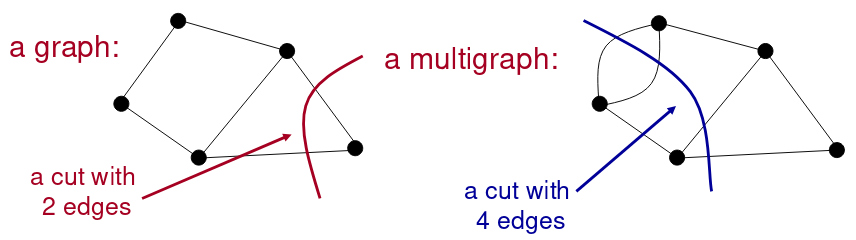
\includegraphics[scale=0.7]{Aggregate1}
	\end{center}
	\item A cut in a (multi)graph is a set of edges whose removal disconnects it
	\item The min-cut problem: given a multigraph, find a cut with the fewest edges
	\item There exist efficient deterministic algorithms using "network flows"
	\item Lets try randomisation - a really simple algorithm
	\item First, an easy observation:
	\begin{itemize}
		\item Let S be a min-cut of a multigraph
		\item If S has an edge between vertices a and b then S has all edges between a and b
		\item Why? Since otherwise there exists a smaller cut
	\end{itemize}
	\item Contraction of an edge $e=(u,v)$:
	\begin{itemize}
		\item merge $u$ and $v$ into a single new vertex "$uv$"
		\item all edges between u and v disappear
		\item any other edge $(w,u)$ or $(w,v)$ of the old vertices $u,v$ becomes an edge $(w,"uv)$ of the new vertex $"uv"$
	\end{itemize}
\end{itemize}
\begin{center}
	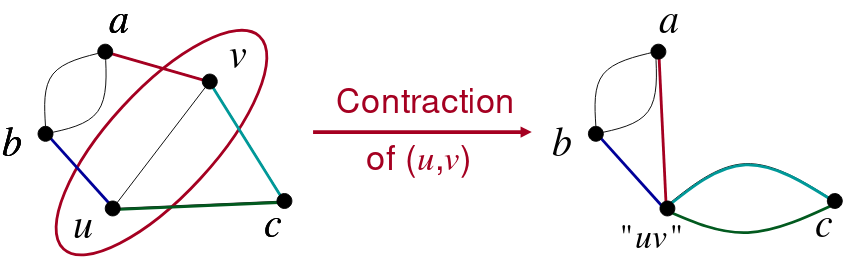
\includegraphics[scale=0.7]{contraction}
\end{center}
\begin{itemize}
	\item A simple Monte Carol algorithm:
	\begin{itemize}
		\item pick randomly an edge and contract it
		\item iterate until only two vertices remain
		\item return the number of edges between these two vertices
	\end{itemize}
	\item At every step of the algorithm
	\begin{itemize}
		\item decrease the number of vertices by one
		\item $\Rightarrow$ n-2 iterations for a graph with $n$ vertices
	\end{itemize}
	\item Does this algorithm \textbf{always} find a min-cut? Not always
	\item An edge contraction
	\begin{itemize}
		\item does not reduce the size of a min cut
		\item sometimes it may increase it
	\end{itemize}
	\item Why?
	\begin{itemize}
		\item every cut of the graph after the contraction was also a cut before the contraction, not the inverse
	\end{itemize}
\end{itemize}
\begin{center}
	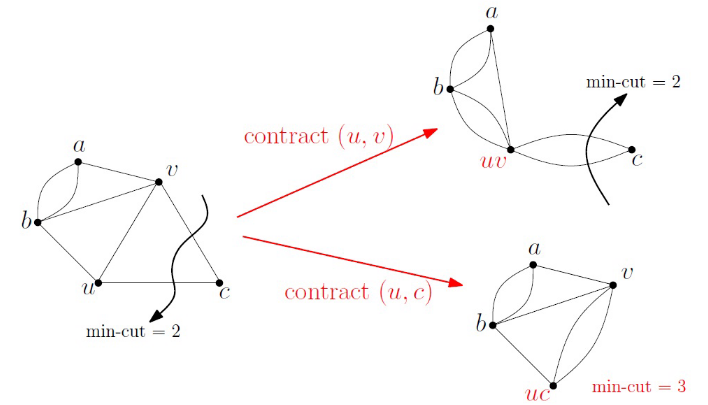
\includegraphics[scale=0.7]{min-cut}
\end{center}
\section{The algorithm in action}
\begin{center}
	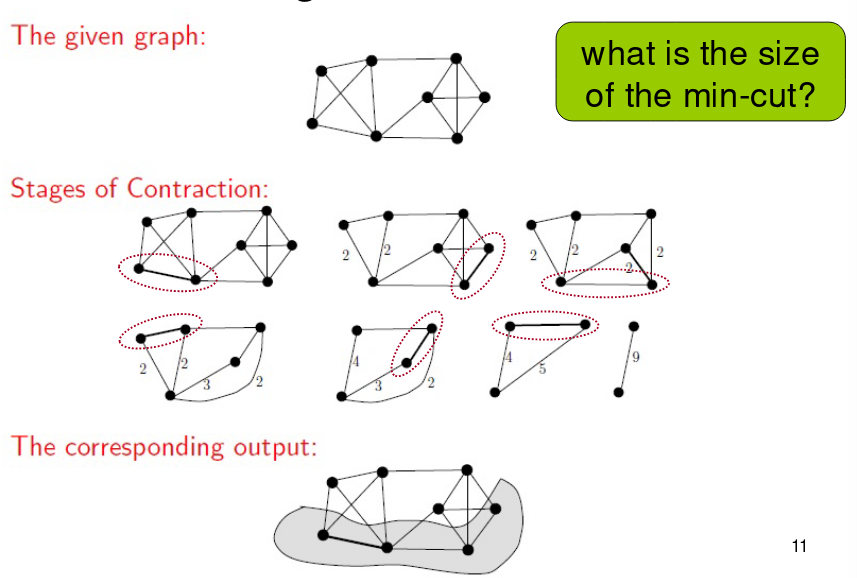
\includegraphics[scale=0.7]{in_action}
\end{center}
\section{How good is the solution}
\begin{itemize}
	\item The input graph has n vertices
	\item suppose that the min-cut S has k edges
\end{itemize}
Lemma: the graph has at least $kn/2$ edges\\
Proof:
\begin{itemize}
	\item If there is a vertex v with less than k neighbours then there is a cut with less than k edges
	\item This is a contradiction, since the min-cut has k edges and all the vertices of the graph have at least k neighbours
	\item Now count the neighbours of all vertices and the graph has at least $kn/2$ edges
\end{itemize}
Thus:
\begin{itemize}
	\item If we pick randomly an edge in the input graph, this edge will belong to the min cut S with probability at most $\dfrac{k}{nk/2}=\dfrac{2}{n}$
	\item This random edge will not belong to the min cut S with probability at least $1-\dfrac{2}{n}$
\end{itemize}
After i iterations (i.e. i contractions)
\begin{itemize}
	\item the current graph has n-i vertices
	\item suppose that we did not contract yet any edge of the min cut S
\end{itemize}
Then, similarly:
\begin{itemize}
	\item If we pick randomly an edge in the current graph, this edge will belong to the min cut S with probability at most $\frac { k } { ( n - i + 1 ) k / 2 } = \frac { 2 } { ( n - i + 1 ) }$
	\item This random edge will not belong with the min cut S with probability at least $1 - \frac { 2 } { ( n - i + 1 ) }$
\end{itemize}
Summarising:
\begin{itemize}
	\item During all (n-2) iterations of the algorithm, we did not contract any edge of the min cut S with probability at least
\end{itemize}
$$\left( 1 - \frac { 2 } { n } \right) \cdot \left( 1 - \frac { 2 } { n - 1 } \right) \cdot \left( 1 - \frac { 2 } { n - 2 } \right) \cdot \left( 1 - \frac { 2 } { n - 3 } \right) \cdots \left( 1 - \frac { 2 } { 4 } \right) \cdot \left( 1 - \frac { 2 } { 3 } \right)$$
$$= \left( \frac { n - 2 } { n } \right) \cdot \left( \frac { m - 3 } { n - 1 } \right) \cdot \left( \frac { n - 4 } { n - 2 } \right) \cdot \left( \frac { n - 5 } { n - 3 } \right) \cdots \left( \frac { 2 } { 4 } \right) \cdot \left( \frac { 1 } { 3 } \right)$$
$$= \frac { 2 } { n ( n - 1 ) } \geq \frac { 2 } { n ^ { 2 } }$$
That is:
\begin{itemize}
	\item At the end of the algorithm, the min-cut S is found with probability at least $\dfrac{2}{n^2}$
	\item The min cut S is not found with probability at most:
	$$1-\dfrac{2}{n^2}$$
	\item We run this algorithm $x$ times
	\item keep the smallest cut that we found
	\item The probability that after x times we do not detect the min cut is at most $\big(1-\frac{2}{n^2}\big)^x$ (too small)
\end{itemize}
\section{The sorting problem}
The sorting problem:
\begin{itemize}
	\item Given a set of n numbers, sort them in increasing order
	\item Many algorithms, the most widely used: quick-sort
	\begin{itemize}
		\item Choose a pivot $y\in S$
		\item Partition the elements of $S-y$ into two subsets $S_1,S_2$
		\begin{itemize}
			\item every element of $S_1$ is smaller than $y$
			\item every element of $S_2$ is larger than y
		\end{itemize}
		\item recursively sort the sets $S_1$ and $S_2$
		\item output:
		\begin{itemize}
			\item Sorted $S_1$, followed by $y$, followed by sorted $S_2$
		\end{itemize}
	\end{itemize}
\end{itemize}
The main idea of quick-sort: divide and conquer
\begin{itemize}
	\item Try to find an element y that splits $S-y$ into two sets $S_1$ and $S_2$ of the same size
	\item We need to solve two instances of the half size
	\item If we choose the worst pivot
	\begin{itemize}
		\item i.e.always too large/too small pivot
		\item We need $\mathcal{O}(n^2)$ time for a set S with n numbers (all possible comparisons)
	\end{itemize}
	\item If we always choose the best pivot:
	\begin{itemize}
		\item i.e. always a pivot in the "middle"
		\item We need $\mathcal{O}(n\log n)$ time
	\end{itemize}
	\item We get the same running time $\mathcal{O}(n\log n)$
	\begin{itemize}
		\item even if $S_1$ and $S_2$ have almost the same size
	\end{itemize}
	\item This gives us hope
	\begin{itemize}
		\item In every set S of n elements, there exist $n/2$ elements $y$ that split $S-y$ into two almost equal parts
	\end{itemize}
	\item In other words:
	\begin{itemize}
		\item If we randomly pick one element $y$, it will be a "good pivot" with probability $\frac{1}{2}$
	\end{itemize}
	\item Randomised quick sort
	\begin{itemize}
		\item exactly as the standard quick sort
		\item but randomly choose the pivot at every step
	\end{itemize}
\end{itemize}
\section{Randomised Quick-Sort}
\begin{itemize}
	\item Always the correct answer (a sorted sequence)
	\begin{itemize}
		\item no matter which pivot we chose at every step
		\item our choices influence only the running time
		\item a Las Vegas algorithm
	\end{itemize}
	\item The running time is a random variable: the number of comparisons
	\item For every $1\leqslant i, j\leqslant n$ define the random variable:
	\begin{itemize}
		\item $X_{i,j}$ equals 1 if the ith and jth largest elements of S are being compared at some iteration
		\item $X_{i,j}$ equals 0, otherwise
	\end{itemize}
	\item The expected running time is $E \left[ \sum _ { i = 1 } ^ { n } \sum _ { j = i + 1 } ^ { n } X _ { i , j } \right]$
	\item By linearity of expectation, this equals:
	$$\sum _ { i = 1 } ^ { n } \sum _ { j = i + 1 } ^ { n } E \left[ X _ { i , j } \right]$$
	\item We can prove that $E \left[ X _ { i , j } \right] = \frac { 2 } { j - i + 1 }$
	\item Using that, we can prove that the expected running time is $\mathcal{O}(n\log n)$
	\item Random Quick-Sort is expected to perform as a Quick Sort that always chooses a "good" pivot
\end{itemize}

\end{document}